\documentclass{beamer}
\usepackage[utf8]{inputenc}
\usepackage{verbatim}
\usepackage{tikz}
\usepackage{hyperref}
\usepackage{graphicx}
\usepackage{hyperref}
\setbeamertemplate{footline}[frame number]
\title{Intro to SQL}
\author{\texorpdfstring{Heide Jackson \newline\url{heidej@umd.edu}}{Author}}
\institute{University of Maryland Population Research Center}

\date{August 2019}

\begin{document}
\maketitle
\begin{frame}{High Level Things to Know}
\begin{itemize}
\item SQL (sometimes pronounced SEQUEL or SQL) is a relational database language used for accessing and manipulating data.
\item This presentation will focus on showing how SQL can be called in a SAS environment.
\end{itemize}
\end{frame}


\begin{frame}[fragile]{Why Use SQL with SAS}

\begin{item}
\item By default, manipulation of SAS data within columns can be clunky, limited and not intuitive.
\item SQL offers easy ways of manipulating data within columns.
\item SQL is also great for subsetting data and complex data merges.
\end{item}
\end{frame}

\begin{frame}[fragile]{Calling SQL in SAS}
\begin{itemize}
    \item SQL can be used to load in and create data sets just like a data statement
    \begin{verbatim}
    data savedata;
    set loaddata;
    run;
    /*Same as*/
    proc sql;
    create table savedata as /*Make new data set*/
    select * /*Keep all variables*/
    from loaddata; /*The set statement piece*/
    quit;
    \end{verbatim}
\end{itemize}
\end{frame}
\begin{frame}[fragile]{Manipulating Data}{An Example Where SQL Clearly Beats Base SAS}
\begin{small}
\begin{verbatim}
/*How we could calculate number of hits per team 
and number of players per team in base sas*/
proc sort data=baseball;
by team;
run;
data baseball2; set sashelp.baseball;
by team;
  if first.team then do;
    hitspteam=nhits;
    count_identifier=1;
  end;
  else do;
    hitspteam+nhits;
    count_identifier+1;
  end;
  if last.team then output;
run;
\end{verbatim}
\end{small}
\end{frame}
\begin{frame}[fragile]{Manipulating Data}{An Example Where SQL Clearly Beats Base SAS}
\begin{verbatim}
proc sql;
create table baseballsql as 
select * /*keep all variables*/, 
sum(nhits) as hitspteam, /*Sums number of hits*/
count(team) as count_identifier /*Counts number on team*/
from sashelp.baseball 
group by team; 
/*Indicates that transformations on team level*/
quit;
\end{verbatim}
\end{frame}
\begin{frame}[fragile]{Subsetting Data Using SQL}
\begin{itemize}
    \item SQL allows data to be easily subsetted via the where statement.
\item The where statement can handle multiple conditions and read across data sets.
\begin{verbatim}
proc sql;
create table check as
select *
from sashelp.baseball
where nhits>40;
quit;
\end{verbatim}
\end{itemize}
\end{frame}
\begin{frame}[fragile]{Merging Data Using SQL}
\item SQL can also handle complex merges across multiple data sets.
\item This can be done in combination with other data manipulation.
\begin{verbatim}
    proc sql;
    create table merged as
    /*Select can be used to specify subsets
    from different data sources */
    select a.* b.hitspteam 
    from sas.baseball as a, baseballsql as b
    where a.team=b.team and nhits<100;
    quit;
\end{verbatim}
\end{frame}

\begin{frame}{Other Types of Merges}
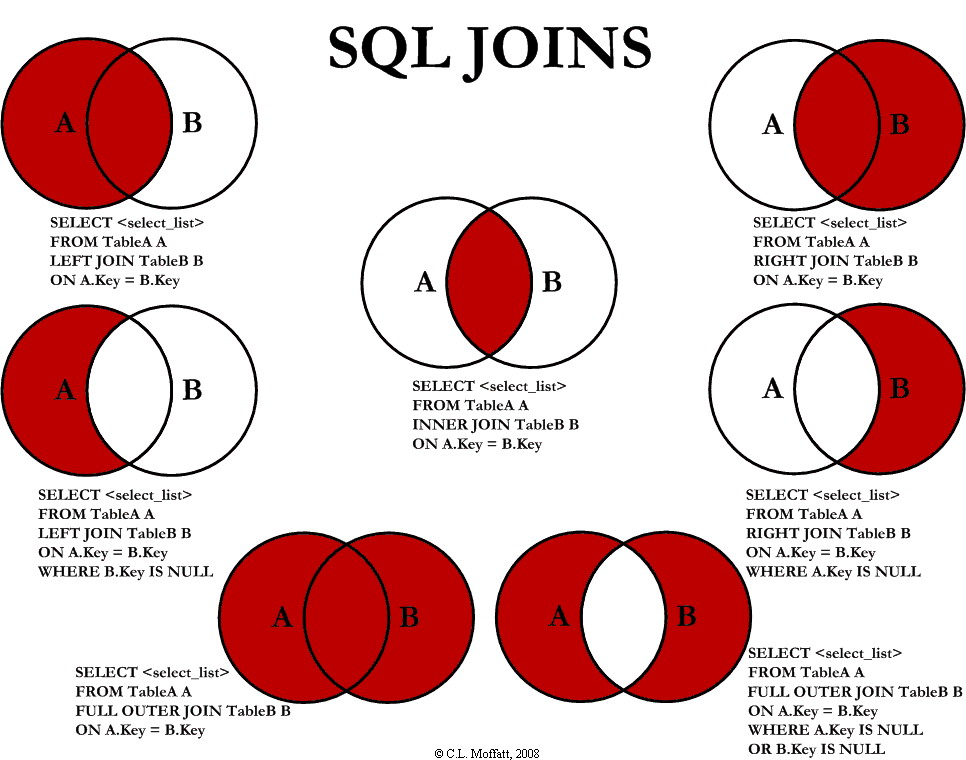
\includegraphics[width=.8\linewidth]{SQL_joins.jpg}
\begin{tiny}
\linebreak
source: \url{https://www.codeproject.com/Articles/33052/Visual-Representation-of-SQL-Joins}
\end{tiny}
\end{frame}

\end{document}
